\section{Interest Flooding in NDN}
\label{sec:interest flooding}

Any DoS attack aims to exhaust system resources. In the context of NDN by term "system" we understand two things: 1) every individual NDN router 2) a distributed system consisting of some collection of NDN routers. In a first case, every major data structure (FIB, CS, PIT) is a potential surface for denial of service attack. In a second case, we consider: 1) bandwidth between NDN routers 2) caching capabilities of NDN routers 3) packet processing capabilities of NDN routers.

Let's examine an individual NDN router first. Certainly, as any other piece of software each specific NDN implementation can have bugs and exploits e.g. buffer overflows leading to data corruption in cache, etc. In this paper we are assuming an idealized NDN implementation lacking any implementation bugs. 

In a general case, Forwarding Interest Base (FIB) is managed by routing protocol and if attackers have been able to get control over routing, they could advertise a huge number of FIB announcements that will fill up FIB table that may cause Interest processing delays and traffic redirection with amplification or black-holing.

Pending Interest Table (PIT) is used to keep per packet forwarding state in NDN and is critical for Data delivery. Though PIT table has an upper limit on its size, it doesn't prevent attacker from injecting a huge number of false Interest packets at a very high rate, which eventually will lead to a situation where the whole PIT table is full of false Interest packets and is not able to keep forwarding state of Interests coming from legitimate users. This attack may look similar to TCP SYN-flood attack and we call it Interest flooding. 

Content Store (CS) is an effective obstacle for several types of DDoS attacks. CS possesses two important characteristics: maximum size and replacement policy. However, by knowing replacement policy attacker can construct a specific traffic generator that is using weaknesses of a chosen replacement procedure that will lead to increased processing time, slower packet delivery and in some cases de facto a complete inability to cache legitimate data. 

An infrastructure consisting of NDN routers is vulnerable to the following types of attacks: 
\begin{enumerate}
\item Interest flooding. 
\item fkjgkfjgkfg
\end{enumerate} 
%\begin{figure}[htpb]
%  \centering
%  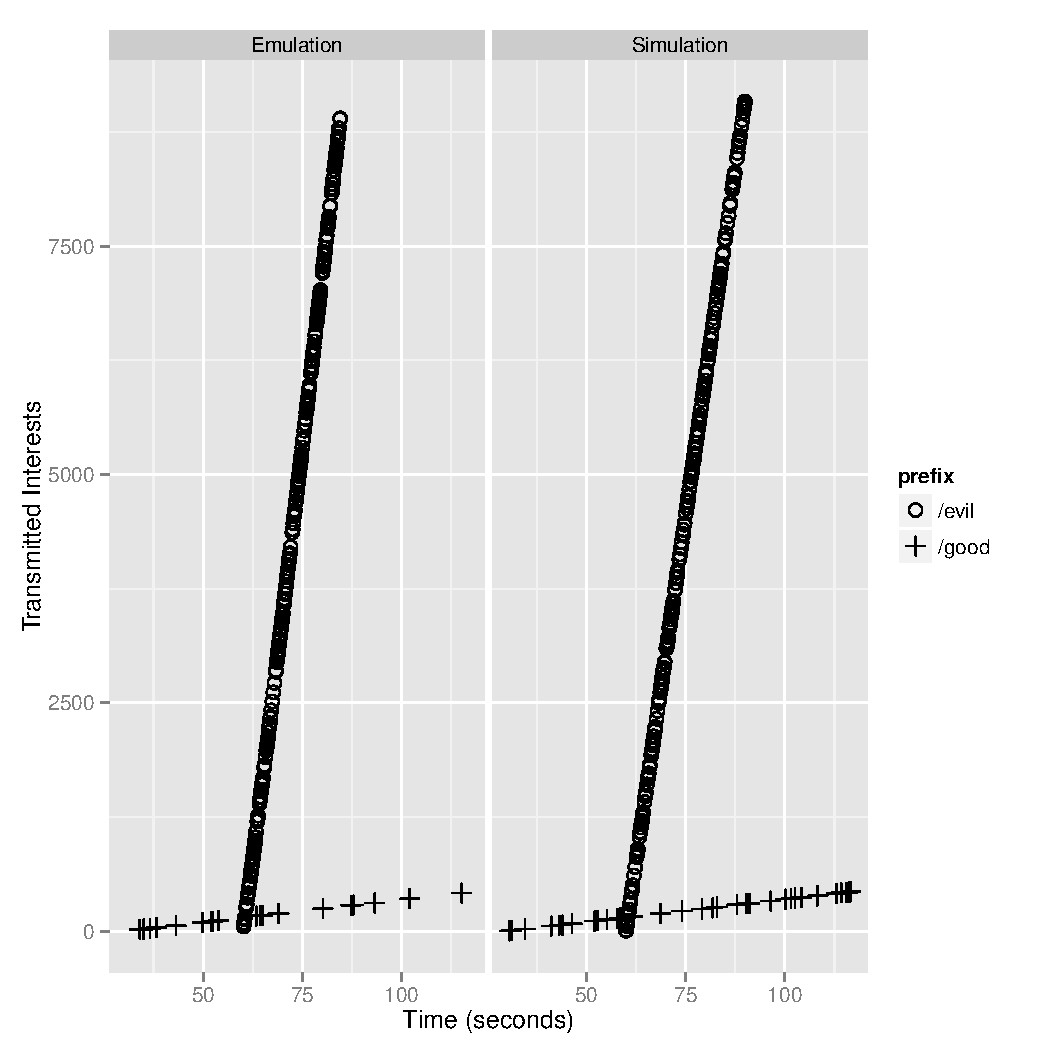
\includegraphics[scale=0.5]{figures/sim-emu-power.pdf}
%  \caption{Strength of Interest flooding attack}
%  \label{fig:simemupower}
%\end{figure}

%\begin{figure}[htpb]
%  \centering
%  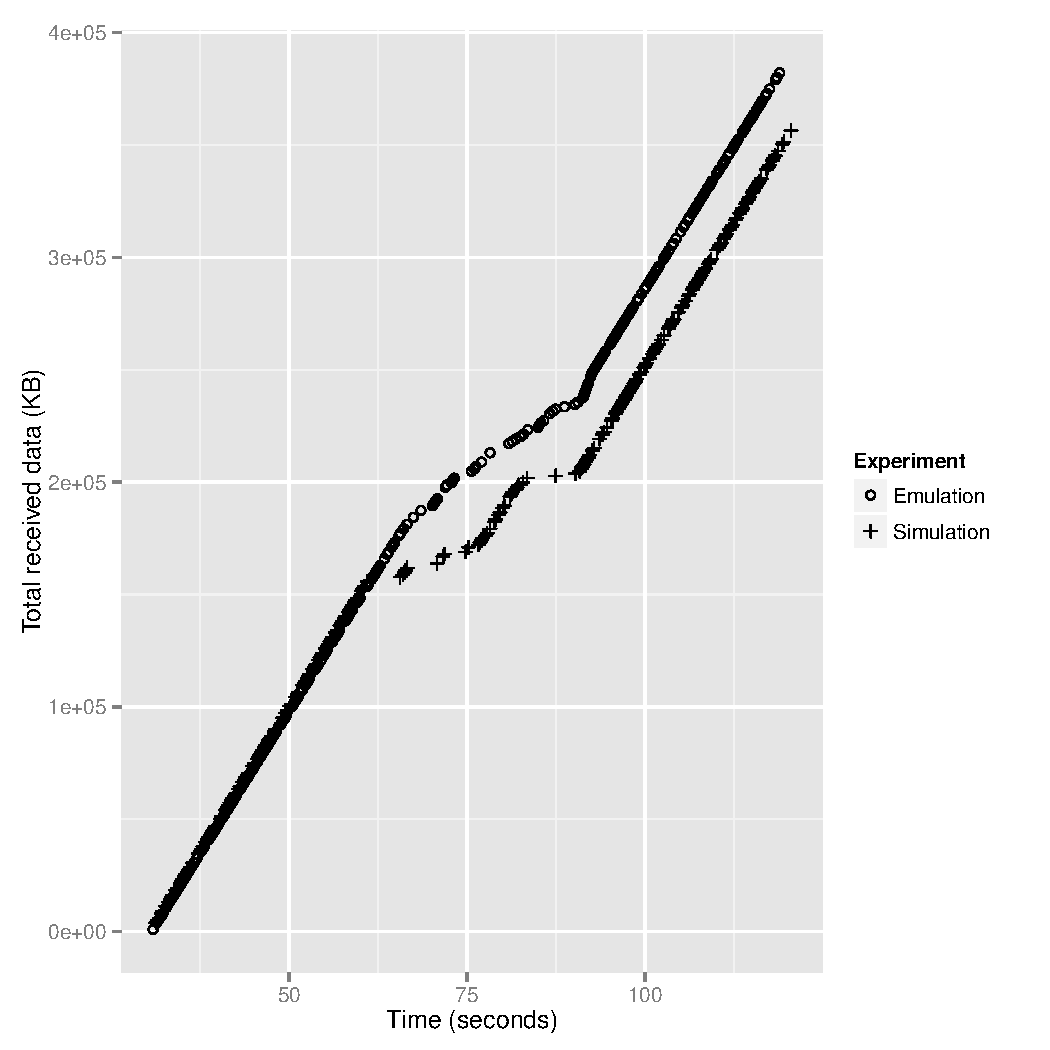
\includegraphics[scale=0.5]{figures/sim-emu-performance.pdf}
%  \caption{Data retrieval by legitimate clients}
%  \label{fig:simemuperf}
%\end{figure}

